\documentclass[pdflatex,sn-mathphys-num]{sn-jnl}

\usepackage{graphicx}
\usepackage{multirow}
\usepackage{amsmath,amssymb,amsfonts}
\usepackage{xcolor}
\usepackage{textcomp}
\usepackage{booktabs}
\usepackage{tabularx}
\usepackage{tikz}
\usetikzlibrary{positioning,arrows.meta,fit,backgrounds}
\usepackage[T1]{fontenc}

\definecolor{press}{HTML}{1E8A8A}
\definecolor{bsky}{HTML}{1D6FD8}
\definecolor{navy}{HTML}{14213D}
\newcommand{\press}{\textcolor{press}{\textsf{press}}}
\newcommand{\bsky}{\textcolor{bsky}{\textsf{Bluesky}}}

\raggedbottom

\begin{document}

\title[Emerging topics in Lyon's press and on Bluesky]{Same Shocks, Different Lenses: Detecting Emerging Topics in Lyon's Local Press and on Bluesky}

\author[1]{\fnm{L\'eo} \sur{Marnas}}
\author[1]{\fnm{Simon} \sur{Hue}}
\author[1]{\fnm{Aaron} \sur{Berton}}

\affil[1]{\orgdiv{D\'epartement Informatique (5IF)}, \orgname{INSA Lyon}, \orgaddress{\city{Villeurbanne}, \country{France}}}

\abstract{\textbf{Project.} 5IF Text Mining / NLP project, INSA Lyon, November 2026. \textbf{Team:} L\'eo Marnas, Simon Hue, Aaron Berton.\\[4pt]
\textbf{Summary.} What becomes newsworthy in a city, when, and through which lens? We study this question for Lyon over thirteen weeks (3 August -- 1 November 2026) by building two comparable corpora: 4,936 headlines from the three local outlets indexed by GDELT, and 4,878 French-language Bluesky posts about the Lyon area. Both were hard to obtain: the GDELT search API was unusable, so we rebuilt the press corpus from raw GDELT files; Bluesky offers no history through its live stream, its unauthenticated search API does not paginate, and a single automated account produced 40\% of the raw posts. On each source we cluster texts into themes (TF-IDF with K-Means, LDA, BERTopic) and detect emerging terms with explainable burst scores that separate \emph{emerging} from merely \emph{frequent} words. We then join the two sources in a shared multilingual embedding space. A joint topic model shows that both sources share most of their agenda (shared topics hold 74\% of press headlines and 71\% of posts), yet only about 5\% of documents have a close counterpart in the other source. Major local shocks (17 October riots, curfew, protest bans, a fatal virus case) peak in both sources within the same one to three days, with no systematic lead of one source over the other. The difference lies in the lens: Bluesky mentions national political actors three to five times more often and frames the same protests mainly through far-right threat and police repression, whereas local headlines favour an order-and-security and local-officials frame. All results are checked with stability analyses, bootstrap intervals, sensitivity tests and manual annotation.}

\keywords{Emerging topic detection, Local news, Bluesky, GDELT, BERTopic, Agenda comparison, Framing}

\maketitle

%% =====================================================================
\section{Introduction}\label{sec:intro}

Local news is where most people meet public life: a fire in their district, a strike on their tram line, an annulled municipal election. In 2026 the local news cycle no longer belongs to newspapers alone. Residents, activists, associations and automated accounts also publish about their city on social networks. Among them, Bluesky, a decentralised network built on the AT Protocol~\cite{kleppmann2024bluesky}, has attracted a large French-speaking audience. Two questions follow for a text-mining project. First, can we detect automatically which local topics \emph{emerge}, meaning they suddenly gain attention, rather than which ones are simply always present? Second, do professional newsrooms and a social network pay attention to the same topics, at the same time, and in the same way?

We address both questions for the Lyon metropolitan area over thirteen weeks (3 August -- 1 November 2026). The period was eventful: a high-school protest movement with blockades and clashes, riots on 17 October followed by a curfew in the city centre, bans on demonstrations, the annulment of municipal elections in two suburbs, and a first human death from the Shamonda virus. It is therefore a good test bed for emergence detection.

\paragraph{Challenges.} Four difficulties shaped the project. \emph{(i) Data access.} We planned to collect local news with the GDELT DOC~2.0 API~\cite{gdeltdoc2017}, but it returned rate-limit errors or empty answers. Only three of the seven targeted Lyon outlets turned out to be indexed. On Bluesky, the live stream gives no history and the unauthenticated search API does not paginate. \emph{(ii) Short and noisy texts.} We only have headlines (about seven informative words each) and short posts, which defeats classic probabilistic topic models~\cite{hong2010twitter,yan2013btm}. \emph{(iii) Unequal and evolving sources.} One regional newspaper dominates the press corpus, one automated account dominates raw Bluesky data, and GDELT has a coverage gap. A naive count would turn these artefacts into ``trends''. \emph{(iv) No ground truth.} Neither themes nor emerging events are labelled, so evaluation must combine internal metrics, external proxies and manual annotation.

\paragraph{Data.} The final material consists of 4,936 press headlines (Le Progr\`es, Lyon Capitale, LyonMag, BFM Lyon) and 4,878 Bluesky posts in the same window, plus 892 Bluesky posts from the preceding month used only as a baseline for emergence scores (Section~\ref{sec:data}).

\paragraph{Research questions and contributions.}
\begin{itemize}
\item[\textbf{RQ1}] Which themes structure Lyon's local news, and which of them \emph{emerge}? We propose a weekly, outlet-weighted burst score for the press and show that it separates emerging from frequent terms.
\item[\textbf{RQ2}] Do the press and Bluesky share the same agenda? We fit a joint topic model in a shared multilingual embedding space and measure each topic's over-representation in each source.
\item[\textbf{RQ3}] Who talks first? We apply the same daily emergence detector to both sources and compare peak dates and first mentions at hour resolution.
\item[\textbf{RQ4}] Do the two sources frame the same events differently? We compare political-actor mentions, frame lexicons, distinctive vocabulary and sentiment.
\end{itemize}

%% =====================================================================
\section{State of the art}\label{sec:sota}

\paragraph{Topic detection and tracking, bursts and emergence.} Detecting new events in news streams was formalised by the Topic Detection and Tracking programme~\cite{allan1998tdt}. Kleinberg modelled bursts as state changes of an automaton~\cite{kleinberg2003bursty}. Fung et al.\ proposed parameter-free bursty-feature detection~\cite{fung2005bursty}. On social media, TwitterMonitor detects bursty keywords and groups them into trends~\cite{mathioudakis2010twittermonitor}, and EDCoW uses wavelet signals of words~\cite{weng2011edcow}. These methods share the idea we reuse: a term \emph{emerges} when its frequency departs from its own recent baseline, not when it is frequent. They were designed for large, homogeneous streams, however. With a few thousand short documents from very unequal sources, the main risk is to detect artefacts of source composition, which these papers do not address.

\paragraph{Topic models for short texts.} LDA~\cite{blei2003lda} assumes long documents with many word co-occurrences. On tweets or headlines its topics degrade~\cite{hong2010twitter}, which motivated short-text models such as the biterm topic model~\cite{yan2013btm}. Vector-space approaches use TF-IDF weighting~\cite{salton1988tfidf}, optionally reduced by latent semantic analysis~\cite{deerwester1990lsa}, then clustered with K-Means. They remain lexical: two headlines about the same event that share no word stay apart. BERTopic~\cite{grootendorst2022bertopic} replaces words by sentence embeddings~\cite{reimers2019sbert,reimers2020multilingual}, reduces them with UMAP~\cite{mcinnes2018umap}, clusters them with HDBSCAN~\cite{campello2013hdbscan} and names clusters with a class-based TF-IDF and Maximal Marginal Relevance~\cite{carbonell1998mmr}. It handles short texts better but leaves many documents unassigned and is sensitive to random seeds. Topic quality is usually measured with coherence (NPMI)~\cite{bouma2009npmi,roder2015coherence}, silhouette~\cite{rousseeuw1987silhouette}, or agreement between partitions (ARI, AMI)~\cite{hubert1985ari,vinh2010ami}, none of which measures journalistic relevance.

\paragraph{News media versus social media.} Kwak et al.\ showed that Twitter behaves partly as a news medium~\cite{kwak2010twitter}. Zhao et al.\ compared Twitter and the \emph{New York Times} with topic models and found different topic mixes~\cite{zhao2011comparing}. Petrovi\'c et al.\ asked whether Twitter can replace newswire for breaking news and found that it covers most newswire events, often slightly earlier~\cite{petrovic2013newswire}. Meme-tracking studies measured the lag between news sites and blogs~\cite{leskovec2009memetracker}. On the communication-science side, agenda-setting~\cite{mccombs1972agenda} and framing~\cite{entman1993framing} theories distinguish \emph{what} is covered from \emph{how} it is covered. Lexical contrast with the informative-prior log-odds of Monroe et al.~\cite{monroe2008fightin} is a standard tool to find words that distinguish two corpora.

\paragraph{Bluesky.} Bluesky and the AT Protocol are recent~\cite{kleppmann2024bluesky}. Measurement studies describe its growth, decentralisation and moderation~\cite{balduf2024bluesky}, and its network topology and political polarisation, with a user base leaning left~\cite{quelle2024bluesky}. We found no study of \emph{local} news on Bluesky, nor any comparison with local newspapers.

\paragraph{Data sources and libraries.} GDELT monitors online news worldwide and publishes 15-minute ``Global Knowledge Graph'' (GKG) files~\cite{leetaru2013gdelt}. Its DOC~2.0 API~\cite{gdeltdoc2017} is the usual entry point but has a three-month window and strict rate limits. Bluesky exposes a live event stream (Jetstream) and a search endpoint~\cite{bskyapi}. We used NLTK stop-word lists~\cite{bird2009nltk}, the dictionary lemmatiser simplemma~\cite{barbaresi2023simplemma}, scikit-learn~\cite{pedregosa2011sklearn}, BERTopic and the multilingual MiniLM sentence encoder~\cite{reimers2020multilingual}. For sentiment we used XLM-T~\cite{barbieri2022xlmt}, an XLM-R model~\cite{conneau2020xlmr} fine-tuned on tweets in eight languages including French.

\paragraph{What is missing.} Existing work compares global newswire with Twitter on large corpora, with event lists taken from the newswire. Our setting differs on three points that the literature does not cover: (i) a \emph{local} scale where each source has a few thousand documents and its own biases (a dominant regional paper, dominant bots); (ii) a \emph{decentralised} network without a free historical API; (iii) the need to compare not only timing but also \emph{framing}, without any labelled data. Our contribution is a careful, reproducible pipeline that builds comparable corpora from both sources and joins them in one semantic space, together with explicit controls for the artefacts listed above.

%% =====================================================================
\section{Contribution}\label{sec:contrib}

\subsection{Approach}\label{sec:approach}

Figure~\ref{fig:pipeline} summarises the approach. Each source is first processed on its own (collection, filtering, cleaning, themes, emergence), so that each analysis fits its texts: short headlines for the press, full sentences for Bluesky. The two corpora are then aligned on the same period and the same territorial scope, encoded with the same multilingual sentence model, and compared along four axes: agenda (shared topics), echo (pairs of documents about the same story), timing (synchrony and emergence lags) and framing (actors, frames, vocabulary, sentiment).

\begin{figure}[htbp]
\centering
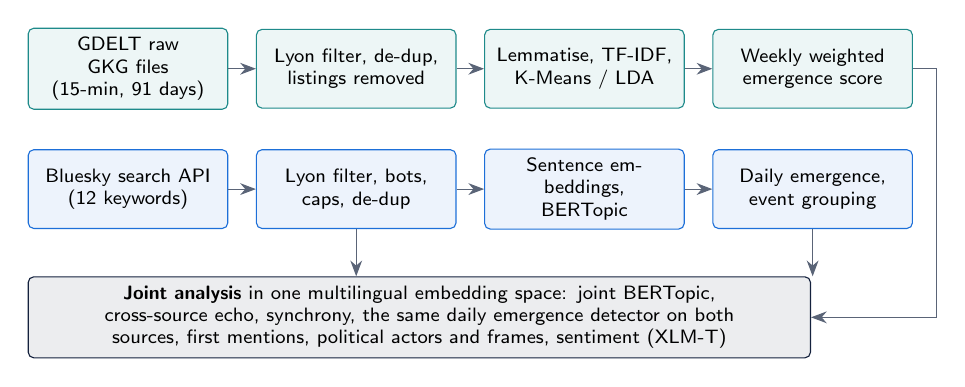
\begin{tikzpicture}[font=\sffamily\scriptsize, node distance=3mm and 3.5mm,
  box/.style={draw=#1, fill=#1!8, rounded corners=2pt, align=center, minimum height=10mm, text width=23mm},
  arr/.style={-{Stealth[length=2mm]}, navy!70}]
\node[box=press] (p1) {GDELT raw GKG files\\(15-min, 91 days)};
\node[box=press, right=of p1] (p2) {Lyon filter, de-dup,\\listings removed};
\node[box=press, right=of p2] (p3) {Lemmatise, TF-IDF,\\K-Means / LDA};
\node[box=press, right=of p3] (p4) {Weekly weighted\\emergence score};
\node[box=bsky, below=5mm of p1] (b1) {Bluesky search API\\(12 keywords)};
\node[box=bsky, right=of b1] (b2) {Lyon filter, bots,\\caps, de-dup};
\node[box=bsky, right=of b2] (b3) {Sentence embeddings,\\BERTopic};
\node[box=bsky, right=of b3] (b4) {Daily emergence,\\event grouping};
\foreach \a/\b in {p1/p2,p2/p3,p3/p4,b1/b2,b2/b3,b3/b4} \draw[arr] (\a) -- (\b);
\node[box=navy, anchor=north west, text width=97mm, minimum height=9mm] (j) at ([yshift=-6mm]b1.south west)
  {\textbf{Joint analysis} in one multilingual embedding space: joint BERTopic, cross-source echo, synchrony, the same daily emergence detector on both sources, first mentions, political actors and frames, sentiment (XLM-T)};
\draw[arr] (b4.south) -- (b4.south |- j.north);
\draw[arr] (p4.east) -- ++(3mm,0) |- (j.east);
\draw[arr] (b2.south) -- (b2.south |- j.north);
\end{tikzpicture}
\caption{Workflow. Each source is processed with methods suited to its texts (top: \press; middle: \bsky), then both are joined in a shared semantic space for the comparison (bottom).}
\label{fig:pipeline}
\end{figure}

\subsection{Datasets}\label{sec:data}

\subsubsection{Local press from GDELT}

\paragraph{Collection.} We first tested the GDELT DOC~2.0 API on each of the seven target domains (Le Progr\`es, Lyon Capitale, Rue89Lyon, LyonMag, BFM Lyon, Tribune de Lyon, Actu Lyon) and on a control outlet (Le Monde). Even with one request every 12 seconds, from two networks, and from a web browser, the API answered ``HTTP 429'' or an empty JSON object, including for the control. We therefore bypassed the API. GDELT publishes a GKG file every 15 minutes. We downloaded the 8,736 files covering 3 August -- 1 November 2026 in memory, kept only the rows whose URL host belongs to a target outlet, and stored one compressed file per day (5\,MB in total). A second obstacle followed: the standard GKG feed contains almost only English-language media (7 French articles out of 54,361 on a test day). French outlets are in the separate ``translation'' feed, which we used. No 15-minute file was missing. Only Le Progr\`es, Lyon Capitale, LyonMag and BFM Lyon appear in GDELT; Rue89Lyon, Tribune de Lyon and Actu Lyon are absent.

\paragraph{Corpus construction.} The 13,999 rows yield 13,998 unique articles after URL normalisation. Titles are extracted from GDELT's \texttt{PAGE\_TITLE} field (100\% present) and decoded from HTML entities. Le Progr\`es is a regional daily covering several departments (Ain, Jura, Loire, \dots). We kept its Lyon-area articles with three explicit rules: the place prefix of the headline (``Villeurbanne. \dots''), Lyon-area words in the title (excluding false friends such as \emph{Bouches-du-Rh\^one} or \emph{canal du Rh\^one au Rhin}), or a GDELT geolocation in Lyon or Villeurbanne. Agenda listings (84) and sponsored content (6) were removed. GDELT gives the \emph{detection} time; for Le Progr\`es we use the publication date contained in the URL when it is within two days of detection. Finally, GDELT almost stopped indexing Le Progr\`es on 12--13 October (11 and 33 articles instead of about 120), which we flag as a coverage gap. Table~\ref{tab:data} gives the resulting statistics.

\subsubsection{Bluesky}

\paragraph{Two collection strategies.} We first built a collector on Jetstream, Bluesky's live event stream~\cite{bskyapi}. It stores in SQLite every post whose declared languages include French, and applies later edits and deletions. A collection on 8 November 2026 yielded 1,000 posts by 603 authors (930 unique cleaned texts). This design is robust and privacy-aware, but a stream only delivers the present: it cannot rebuild the study period, so emergence and comparison with the press are impossible on this sample. We therefore also collected history with the search endpoint (\texttt{searchPosts}), with twelve Lyon keywords (\emph{lyon, lyonnais, villeurbanne, rh\^one, part-dieu, bellecour, croix-rousse, v\'enissieux, tcl}, \dots), language set to French, day by day from 3 July to 1 November 2026. The first month serves only as a baseline for emergence scores.

\paragraph{Collection difficulties.} A first version re-read the same result page in a loop because the pagination cursor was not passed (10,000 rows for about 97 distinct posts). When we re-ran the collection for this report without authentication, page~2 of every result list came back empty. We replaced pagination with \emph{adaptive time splitting}: any time window that returns a full page (100 posts) is split in two, recursively, until each window fits in one page. The re-collection gathered 23,191 posts, 88\% of the 26,282 collected earlier with authentication. The gap is consistent with posts and accounts deleted since. The per-day counts of the first days match within one or two posts.

\paragraph{Corpus construction.} Table~\ref{tab:funnel} shows the funnel. One automated account alone produced 39.8\% of the raw posts. It was excluded together with two other aggregators and five accounts flagged automatically (at least 50 posts with at least 50\% links or at least 30\% duplicates). We also dropped replies (mostly conversational), posts under five words and normalised duplicates, and capped each account at five posts per day. For this report we corrected the territorial filter: 10.6\% of the posts kept by the original rule matched only through \emph{Bouches-du-Rh\^one}, \emph{vall\'ee du Rh\^one} or \emph{Gare de Lyon} (Paris), which brought Marseille and national news into the corpus. The final corpus has 5,770 posts, of which 4,878 fall in the study window, written by 1,603 accounts. The ten most active accounts write 21\% of the posts and 63\% of the accounts post only once.

\begin{table}[htbp]
\caption{The two corpora in the study window (3 Aug -- 1 Nov 2026). Sentiment is predicted by XLM-T (Section~\ref{sec:eval}).}\label{tab:data}
\begin{tabularx}{\textwidth}{@{}lXX@{}}
\toprule
 & \press & \bsky \\
\midrule
Documents analysed & 4,936 headlines & 4,878 posts \\
Producers & 4 outlets: Le Progr\`es 2,171; Lyon Capitale 1,855; LyonMag 832; BFM Lyon 78 & 1,603 accounts \\
Mean length (words) & 14.9 & 29.0 \\
Documents per day (mean) & 54.2 & 53.6 \\
Text available & headline only & full post \\
Timestamp & GDELT detection (URL date for Le Progr\`es) & creation time \\
Negative / neutral / positive (\%) & 55 / 15 / 29 & 40 / 29 / 32 \\
\botrule
\end{tabularx}
\end{table}

\begin{table}[htbp]
\caption{Bluesky corpus construction (search API, 3 July -- 1 November 2026).}\label{tab:funnel}
\begin{tabular*}{\textwidth}{@{\extracolsep\fill}lr}
\toprule
Step & Posts \\
\midrule
Collected (12 keywords, adaptive time splitting) & 23,191 \\
Declared language includes French & 23,032 \\
Mention the Lyon area (original keyword rule) & 19,988 \\
Refined territorial filter (no Bouches-du-Rh\^one, Gare de Lyon, \dots) & 19,400 \\
Without automated accounts, aggregators and replies & 6,254 \\
$\ge$5 words, de-duplicated, $\le$5 posts per account per day & 5,770 \\
\quad of which in the study window (3 Aug -- 1 Nov) & 4,878 \\
\botrule
\end{tabular*}
\end{table}

\paragraph{Comparability.} Figure~\ref{fig:volume} shows that the two corpora have similar daily volumes (54 headlines and 54 posts per day on average). Press volume is stable, while Bluesky volume grows and peaks during the October unrest. The two daily volume series are only weakly correlated ($r=0.32$). For this reason, all comparisons use \emph{shares} of each day's or week's documents, never raw counts.

\begin{figure}[htbp]
\centering
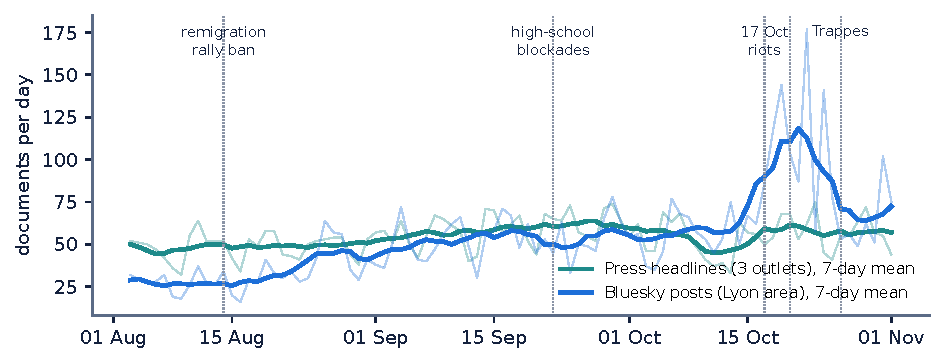
\includegraphics[width=\textwidth]{figures/f1_daily_volume.pdf}
\caption{Daily number of documents in each source (thin lines) and 7-day means (thick lines), with the main events of the period.}
\label{fig:volume}
\end{figure}

\subsection{Workflow}\label{sec:workflow}

\paragraph{Preprocessing.} Press headlines are lower-cased, elisions are removed (\emph{l'ancien} $\rightarrow$ \emph{ancien}), and we drop the NLTK French stop words plus words present in nearly every headline (\emph{lyon}, \emph{rh\^one}, months, numbers). Words are then lemmatised with simplemma (\emph{saisis} $\rightarrow$ \emph{saisir}). This removes 47\% of the tokens and reduces the vocabulary from 9,686 to 7,232 forms; 49\% of the lemmas occur only once, so the data are very sparse. Bluesky posts keep two versions: the full sentence without links, mentions or \texttt{\#} for sentence embeddings, and an accent-free lexical version for counts.

\paragraph{Themes.} \emph{Press:} TF-IDF vectors (sub-linear term frequency; 4,929 headlines $\times$ 2,528 terms, density 0.22\%) are reduced to 100 LSA dimensions and clustered with K-Means. LDA is fitted on raw counts for comparison. \emph{Bluesky:} BERTopic on multilingual MiniLM embeddings (384 dimensions), with UMAP (15 neighbours, 5 dimensions), HDBSCAN (minimum cluster size $\max(15,0.002N)$), c-TF-IDF with MMR keywords, merging of similar topics and re-assignment of outliers to the nearest topic (cosine $\ge 0.35$). \emph{Joint model:} the same BERTopic configuration fitted on the union of both corpora in the study window (9,814 documents), so that topic numbers mean the same thing in both sources. While building it we found that BERTopic, in its default English mode, deletes accented letters from topic keywords (\emph{m\'etropole} became \emph{mtropole}), a problem also present in our first Bluesky model; we switched to the multilingual mode.

\paragraph{Emergence scores.} For the press we use a \emph{weekly} score because Lyon Capitale publishes half as much on weekends, which creates a seven-day cycle. For term $w$ and week $t$, $p_t(w)$ is the share of headlines containing $w$. It is computed per outlet $m$ and recombined with fixed weights $\pi_m$ (the outlets' average shares: 45\%, 38\%, 17\%), so that the October GDELT gap cannot fake a decline:
\begin{equation}
p_t(w)=\sum_m \pi_m\,\frac{n_{m,t}(w)}{n_{m,t}},\qquad
z_t(w)=\frac{p_t(w)-\bar p_{t-4..t-1}(w)}{\sqrt{\sigma^2_t+\sigma^2_{\text{base}}}},
\end{equation}
where the variances are binomial. A term emerges if $z\ge 4$, with at least 6 headlines in the peak week and at least 2 outlets. Terms whose documents overlap with Jaccard $\ge 0.6$ in the same week are merged into one event. For the cross-source comparison we apply one \emph{daily} detector to both sources, the one first designed for Bluesky: observed counts in a 3-day window are compared with the rate of the 28 preceding days, $z=(o-e)/\sqrt{e+1}$, with $z\ge 4$, at least 6 documents and at least 2 distinct authors (outlets for the press). Both corpora are evaluated only from 2 September, the first day for which the press has a full baseline.

\paragraph{Cross-source measures.}
\emph{Agenda overlap:} for each joint topic $k$ we compute $\log_2\!\big(s^{\text{bsky}}_k / s^{\text{press}}_k\big)$, where $s_k$ is the topic's share of each source. A topic is ``source-dominated'' when one source over-represents it at least threefold. We summarise the two topic distributions with the Jensen--Shannon divergence~\cite{lin1991jsd} and compare it with a permutation null in which source labels are shuffled.
\emph{Echo:} each press headline is matched with its most similar Bluesky post (cosine of the embeddings) published within $\pm 2$ days, and vice versa. A pair is an echo above a threshold $\tau$ calibrated by manual annotation.
\emph{Synchrony:} Pearson correlation of the daily topic shares (3-day smoothing) for lags of $-5$ to $+5$ days.
\emph{Framing:} mentions of party families and local actors per 1,000 documents (regular expressions over party names and national leaders only, to avoid uncertain affiliations); five frame lexicons applied to protest-related documents (\emph{order \& security}, \emph{far-right threat}, \emph{police repression}, \emph{social grievance}, \emph{radical-left threat}); and the log-odds ratio with an informative Dirichlet prior~\cite{monroe2008fightin} to find each source's distinctive words within shared topics.

\subsection{Evaluation methods}\label{sec:eval}

Because no labelled data exist, we combine five kinds of evidence.
\begin{enumerate}
\item \textbf{Internal cluster metrics:} silhouette~\cite{rousseeuw1987silhouette} (cosine), stability across random seeds measured by the adjusted Rand index (ARI)~\cite{hubert1985ari}, and NPMI coherence~\cite{bouma2009npmi} for LDA.
\item \textbf{External proxy:} agreement (adjusted mutual information~\cite{vinh2010ami}) between press clusters and the editorial sections of Le Progr\`es found in its URLs (\emph{faits-divers-justice}, \emph{economie}, \dots), available for 44\% of the headlines.
\item \textbf{Manual annotation:} the 32 highest-scoring emerging press terms were checked by reading their peak headlines, and 60 cross-source pairs (15 per similarity band) were labelled ``same story'' or not. Both annotations were done by one annotator, which is a limitation.
\item \textbf{Validity of the sentiment instrument:} on press headlines, the XLM-T polarity ($p_{\text{pos}}-p_{\text{neg}}$) is compared with GDELT's tone, which GDELT computes from the \emph{full article text}. The Spearman correlation is $\rho=0.59$ and mean polarity increases across the five tone quintiles ($-0.73, -0.53, -0.26, 0.03, 0.36$), so the instrument is usable for comparisons.
\item \textbf{Uncertainty and robustness:} 95\% bootstrap intervals~\cite{efron1993bootstrap} on rates, a permutation null for the divergence, a sign test on lags, and sensitivity analyses in which one methodological choice is changed at a time.
\end{enumerate}

\subsection{Experiments and results}\label{sec:results}

\subsubsection{E1 -- Themes and emerging topics in the local press}

\paragraph{Vocabulary.} PMI~\cite{church1990pmi} on bigrams separates true expressions (\emph{gilets jaunes}, PMI 12.3; \emph{refus d'obtemp\'erer}, 11.8) from frequent but banal pairs (\emph{millions euros}, 42 occurrences, PMI 8.8). Log-odds contrasts show distinct outlet profiles: Le Progr\`es over-uses local-life words (\emph{Beaujolais}, \emph{\'ecole}, \emph{habitant}), Lyon Capitale regional alerts (\emph{vigilance}, \emph{Is\`ere}, \emph{Dr\^ome}), and LyonMag politics and security (\emph{mobilisation}, \emph{Doucet}, \emph{policier}).

\paragraph{Themes.} Table~\ref{tab:press_models} compares the press models. The silhouette of K-Means grows with $k$ by construction (from 0.03 to 0.16 between $k=4$ and $k=30$), so it cannot select $k$. We kept $k=14$, the best agreement with Le Progr\`es sections among moderate values of $k$. LDA fails on headlines: its NPMI coherence is negative for every number of topics, and its agreement with the sections is near zero. Figure~\ref{fig:press_themes} shows the weekly share of the main K-Means themes. High-school protests rise from about 4\% to 19\% of headlines in the week of 5 October; municipal politics climbs to 15\% in the week of 19 October.

\begin{table}[htbp]
\caption{Press topic models (4,929 headlines). AMI: agreement with Le Progr\`es editorial sections. The two partitions agree poorly with each other (ARI 0.03).}\label{tab:press_models}
\begin{tabular*}{\textwidth}{@{\extracolsep\fill}lcccc}
\toprule
Model & Silhouette & Stability (ARI) & NPMI & AMI \\
\midrule
TF-IDF + LSA + K-Means ($k=14$) & 0.083 & 0.25 & -- & 0.119 \\
LDA ($k=6$, best coherence) & -- & -- & $-0.17$ & 0.032 \\
\botrule
\end{tabular*}
\end{table}

\begin{figure}[htbp]
\centering
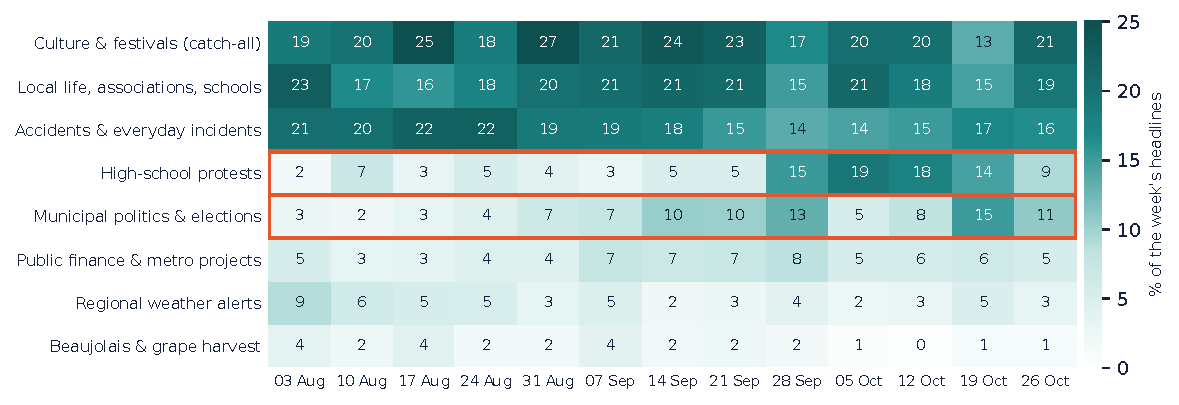
\includegraphics[width=0.95\textwidth]{figures/press_themes_week.pdf}
\caption{Weekly share (\%) of eight of the fourteen press themes (K-Means). Framed rows: the two themes with a significant upward trend.}
\label{fig:press_themes}
\end{figure}

\paragraph{Emergence.} The weekly score flags 87 emerging terms, which merge into 14 events (Figure~\ref{fig:press_events}). Reading the peak headlines, 31 of the 32 top terms correspond to an identifiable event; the only false positive is the generic word \emph{chef}. Three waves appear: institutional news in mid-September (an appeal against the municipal election, the IOC visit for the 2030 Winter Games, the Art Biennale), the high-school protest movement from 28 September to 12 October (40 headlines in the peak week), and a series of shocks in late October (riots and curfew, the Deranque case, the Trappes attack). The score does separate emergence from frequency (Figure~\ref{fig:press_freq}): the rank correlation between a word's total frequency and its highest score is $-0.20$, and the most frequent words (\emph{homme}, \emph{bless\'e}) never cross the threshold.

\begin{figure}[htbp]
\centering
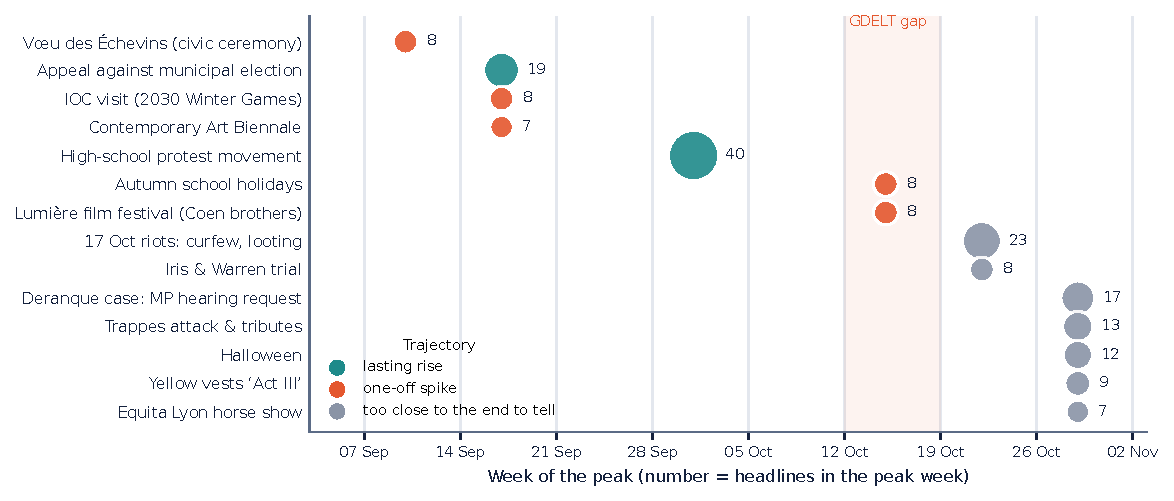
\includegraphics[width=0.95\textwidth]{figures/press_events.pdf}
\caption{The 14 emerging press events, placed at their peak week. Colour: trajectory of the main term after its peak.}
\label{fig:press_events}
\end{figure}

\begin{figure}[htbp]
\centering
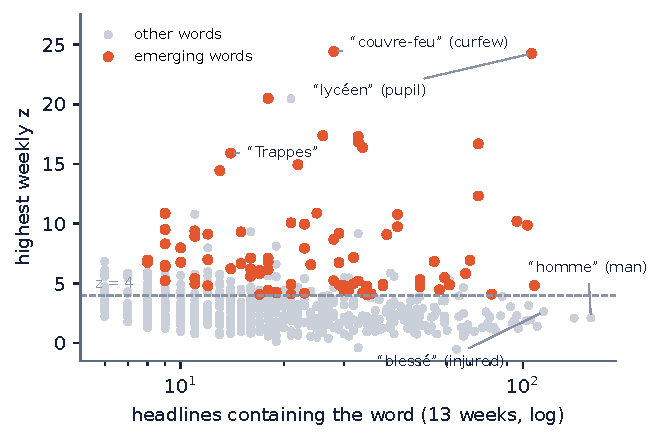
\includegraphics[width=0.6\textwidth]{figures/press_freq_vs_emergent.pdf}
\caption{Frequency is not emergence: total number of headlines containing a word versus its highest weekly score (press, 1,391 lemmas and bigrams).}
\label{fig:press_freq}
\end{figure}

\paragraph{Robustness.} Changing one choice at a time, the set of emerging terms overlaps with the reference with Jaccard 0.97 (without the low-coverage days), 0.89 (without outlet weighting), 0.77 (3-week baseline) and 0.57 (6-week baseline, which leaves only 7 weeks to test). Thresholds of $z\ge 3$ and $z\ge 6$ give nested sets of 126 and 50 terms. The top-20 terms change by at most three words, all variants of the same events. Declining terms are mostly seasonal: \emph{canicule} goes from 43 headlines in the first four weeks to 5 in the last four, and \emph{\'eclipse} and \emph{vendanger} vanish. Thirteen weeks are not enough to separate a seasonal decline from an editorial one.

\subsubsection{E2 -- Topics on Bluesky}

On the first, authenticated collection, BERTopic produced 101 raw topics with 41\% unassigned posts; merging and outlier re-assignment gave 29 topics with 1\% left out. The same TF-IDF + K-Means pipeline used for the press failed on Bluesky: one cluster absorbed 62\% of the posts (4,197 of 6,808) and the silhouette was 0.016, which justifies semantic embeddings for posts. The daily emergence detector found 405 terms grouped into 201 events. They were dominated by the curfew (\emph{couvre-feu}: 107 posts by 92 accounts in three days, $z=103$) and also included football (Europa League, PSG) and national news reached through the Lyon keywords (Limoges, Marseille). This last observation led to the filter correction of Section~\ref{sec:data}. The Jetstream pipeline was also run end to end on its one-day sample (275 posts after analysis filters) and documents explicitly why BERTopic and emergence cannot be computed on such a sample. This is a useful negative result: a live stream must run for months before it supports temporal analysis.

\subsubsection{E3 -- One agenda or two? Joint topic model}

The joint BERTopic model on 9,814 documents yields 109 raw topics (30\% outliers), merged into 39 topics with 0.7\% of documents left out. With other random seeds the partitions agree with ARI 0.52 and 0.64, a moderate stability that leads us to interpret topic groups rather than single topic boundaries. Labels were assigned by reading keywords and sampled documents of each topic.

Figure~\ref{fig:composition} shows each topic's over-representation. 23 topics are \emph{shared} (less than a threefold difference), 9 are Bluesky-dominated and 7 press-dominated. Shared topics hold 74\% of non-outlier press headlines and 71\% of posts. The largest topic, protests, the high-school movement and the curfew, has nearly the same weight in both sources (12.5\% of headlines, 14.5\% of posts). Municipal politics, transport and urban projects, health and climate are also balanced. The press over-represents everyday incidents: accidents and deaths, fires, drownings, trafficking trials and shop damage (log-ratios between $-1.8$ and $-2.7$). Bluesky over-represents sport results, street photography, science events, and two kinds of automated content that our filters did not fully remove (deals and promotions; trending-topic bots). The Jensen--Shannon divergence between the two topic distributions is 0.165, far above the 95th percentile of the permutation null (0.004): the agendas overlap but are not interchangeable.

\begin{figure}[htbp]
\centering
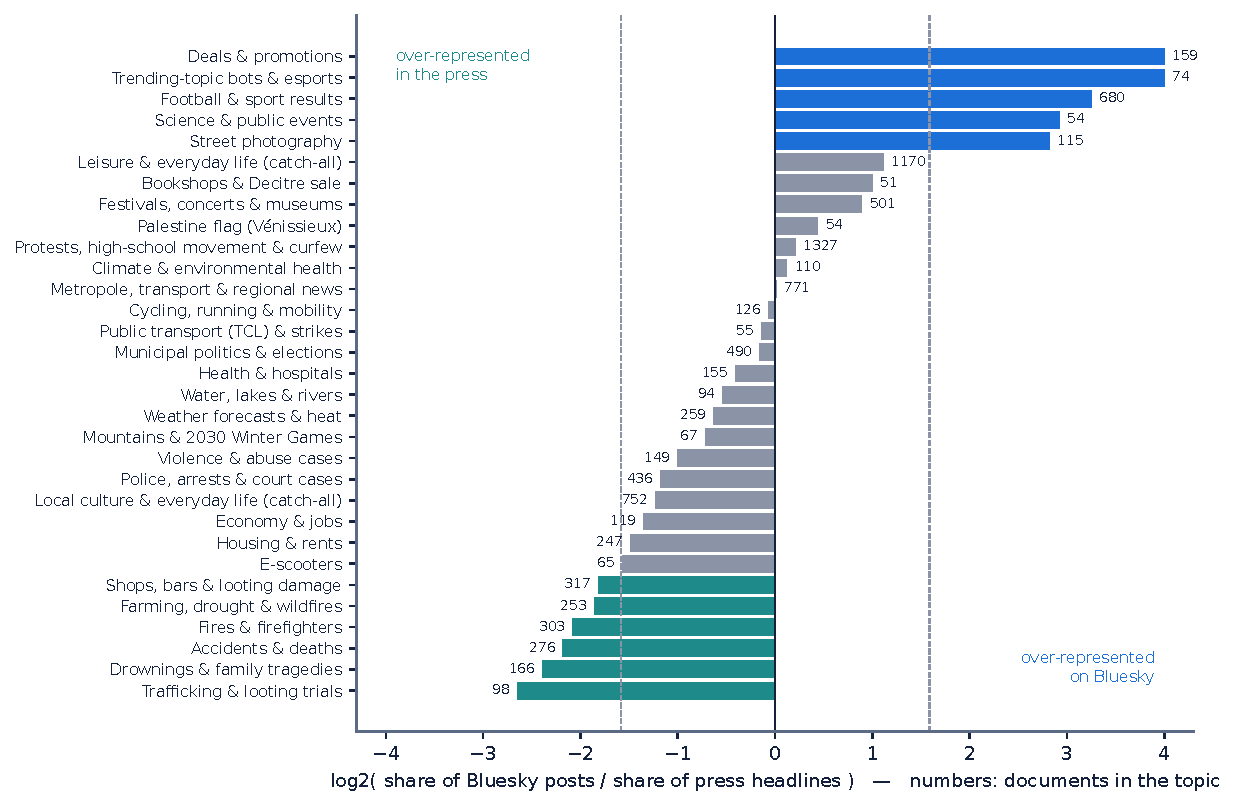
\includegraphics[width=0.92\textwidth]{figures/f2_topic_composition.pdf}
\caption{Joint topic model: over-representation of each topic on Bluesky ($>0$) or in the press ($<0$). Dashed lines: threefold ratio. Numbers: documents in the topic. Topics with at least 50 documents.}
\label{fig:composition}
\end{figure}

\subsubsection{E4 -- Do the two sources tell the same stories? Echo and relays}

Sharing a topic does not mean sharing stories. Figure~\ref{fig:echo}a shows the share of documents whose closest counterpart in the other source, within two days, exceeds a similarity threshold $\tau$. The manual check (Figure~\ref{fig:echo}b) shows that pairs above 0.80 describe the same story in 11 of 15 cases, against 16 of 30 between 0.70 and 0.80 and 4 of 15 below 0.70. At $\tau=0.80$, only 5.5\% of press headlines and 5.1\% of posts are echoed; at $\tau=0.70$, about 17\% (with lower precision). Echo is concentrated on the shocks: 23\% for the Shamonda virus death and 18\% of press headlines on protests, against 1.5\% for Le Progr\`es overall, whose many local items rarely reach Bluesky. LyonMag (11.8\%) and Lyon Capitale (6.8\%) are echoed more. Negative headlines are echoed more often than positive ones (6.4\% versus 3.7\%).

\begin{figure}[htbp]
\centering
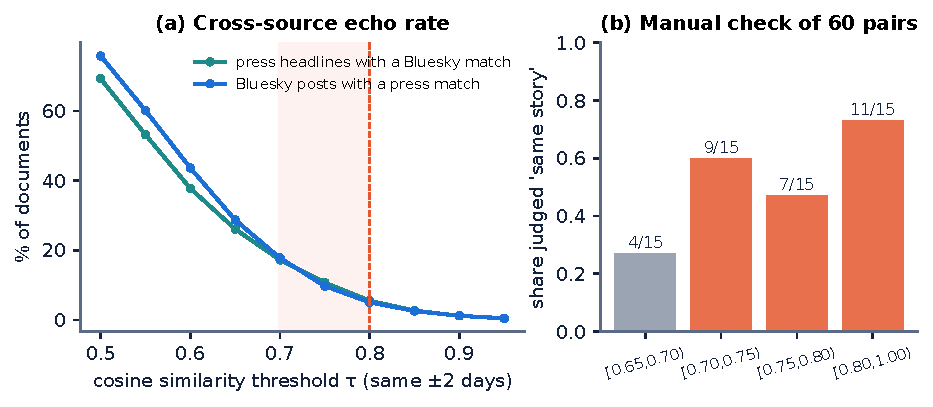
\includegraphics[width=\textwidth]{figures/f3_echo.pdf}
\caption{(a) Share of documents with a semantically close counterpart in the other source within $\pm$2 days, as a function of the cosine threshold. (b) Precision of the matching, judged on 60 annotated pairs.}
\label{fig:echo}
\end{figure}

Links tell a complementary story (Figure~\ref{fig:links}). Among the 16,188 Lyon-related French posts of the window, \emph{before} removing automated accounts, 69\% contain a link. 2,355 posts link to the three studied outlets, but they come from only 84 accounts, and one automated relay account alone publishes 93\% of them. Matching the shared URLs to the press corpus, 1,407 of the 4,936 analysed articles (28.5\%) were posted on Bluesky, nearly all by this relay, and its posts appear a median of 1.0 hour (interquartile range $-1.7$ to $0$ hours) \emph{before} GDELT detects the article. This gives a useful calibration: GDELT's detection time lags publication by roughly one hour, so press ``first mention'' times below are upper bounds. In short, the visible bridge between local newspapers and Bluesky is mostly automated, while human posts rarely reproduce a precise headline.

\begin{figure}[htbp]
\centering
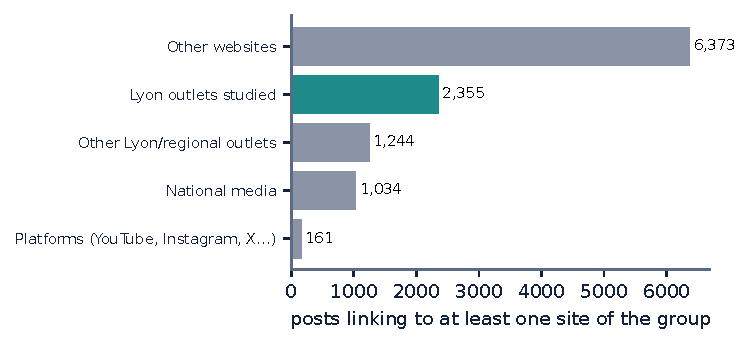
\includegraphics[width=0.55\textwidth]{figures/f9_links.pdf}
\caption{Destinations of links in Lyon-related French Bluesky posts (study window, all accounts).}
\label{fig:links}
\end{figure}

\subsubsection{E5 -- Who talks first? Synchrony and emergence lags}

\paragraph{Synchrony of shared topics.} Daily shares of the big shared topics move together (Figure~\ref{fig:sync}): $r=0.83$ for protests and curfew, $0.75$ for weather and heat, $0.69$ for municipal politics, with best lags of 0 or $+1$ day. For less event-driven topics (housing, local culture) the correlation drops below $0.35$.

\begin{figure}[htbp]
\centering
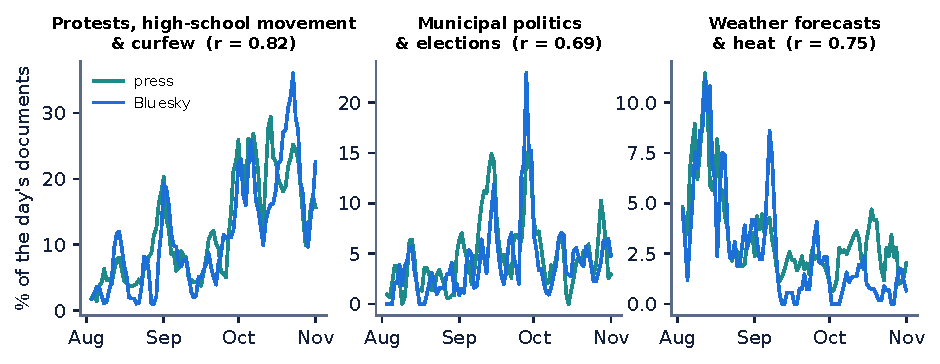
\includegraphics[width=\textwidth]{figures/f4_synchrony.pdf}
\caption{Daily share of three shared joint topics in each source (3-day smoothing) and their same-day correlation.}
\label{fig:sync}
\end{figure}

\paragraph{Emergence with the same detector.} The daily detector finds 122 emerging terms in the press and 261 on Bluesky. 34 terms emerge in both with peaks at most three days apart (Figure~\ref{fig:lags}). Their peak lag has median 0. Bluesky peaks earlier for 13 terms, both peak on the same day for 13, and the press peaks earlier for 8; a sign test on onset dates is not significant ($p=0.11$). In a preliminary run with the original territorial filter (and a looser seven-day matching window), the onsets suggested a significant Bluesky lead (24 of 38 shared terms, $p<0.001$): Marseille and national posts had made Bluesky look ``faster''. This shows how sensitive timing conclusions are to corpus construction.

\begin{figure}[htbp]
\centering
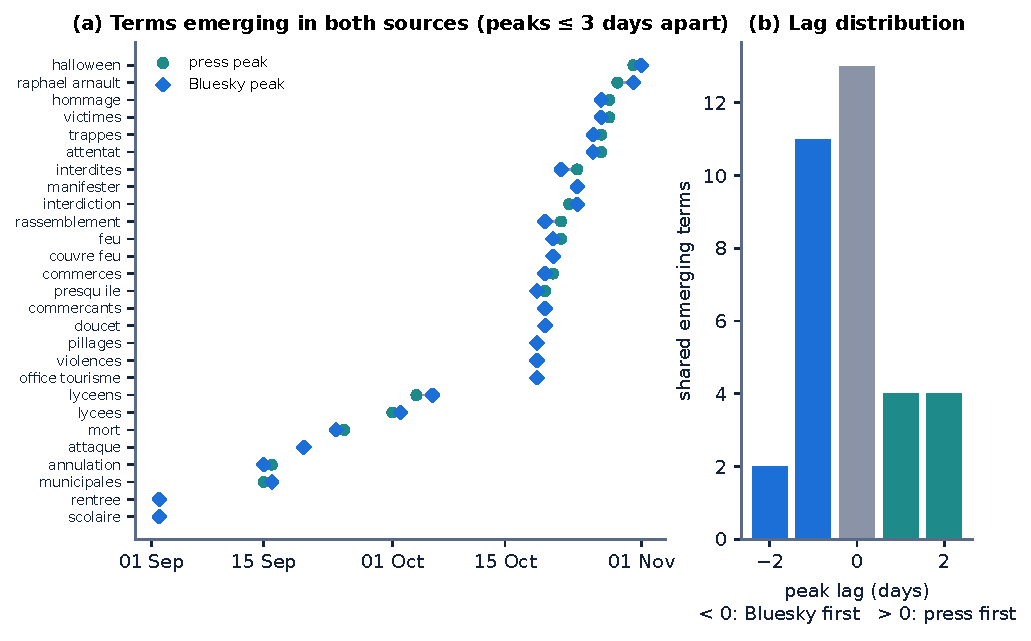
\includegraphics[width=\textwidth]{figures/f5_emergence_lag.pdf}
\caption{(a) Peak dates of the terms that emerge in both sources. (b) Distribution of peak lags (negative: Bluesky first).}
\label{fig:lags}
\end{figure}

\paragraph{First mentions at hour resolution.} Table~\ref{tab:first} compares the first document of each source for eleven events. Bluesky mentions sudden, visible events earlier: the tourist office fire during the 17 October riots ($-3.2$\,h), looting ($-1.4$\,h), the curfew ($-1.9$\,h). Given the roughly one-hour GDELT delay, most of these differences shrink to about one or two hours. The press is first on announced or institutional events: the start of high-school blockades ($+3.8$\,h), the ban on all protests ($+1.9$\,h), the call to ban an ultra-right ``remigration'' rally ($+42$\,h). The press also covers some stories that Bluesky ignores, such as the Deranque family's request for a hearing of an MP. The Trappes attack is a national event that local outlets cover only once there is a local angle (tributes in Lyon), a day after Lyon users discuss it.

\begin{table}[htbp]
\caption{First mention of each event in each source (search window: four days from the given start; press times are GDELT detections, which lag publication by about 1\,h). $\Delta$: Bluesky minus press, in hours.}\label{tab:first}
\begin{tabular*}{\textwidth}{@{\extracolsep\fill}lrrrr}
\toprule
Event & Press & Bluesky & $\Delta$ (h) & Docs (P/B) \\
\midrule
Call to ban ``remigration'' rally & 10 Aug 19:45 & 12 Aug 13:37 & $+41.9$ & 5 / 3 \\
V\'enissieux election annulled & 15 Sep 07:45 & 15 Sep 00:30 & $-7.2$ & 4 / 3 \\
High-school blockades begin & 22 Sep 06:00 & 22 Sep 09:50 & $+3.8$ & 7 / 2 \\
Palestinian flag at V\'enissieux town hall & 22 Sep 11:45 & 22 Sep 12:16 & $+0.5$ & 5 / 2 \\
17 Oct riots: tourist office fire & 17 Oct 16:00 & 17 Oct 12:48 & $-3.2$ & 6 / 15 \\
17 Oct riots: looting & 17 Oct 16:30 & 17 Oct 15:03 & $-1.4$ & 36 / 34 \\
Curfew in the Presqu'\^ile & 19 Oct 18:30 & 19 Oct 16:37 & $-1.9$ & 12 / 66 \\
Ban on all protests (24 Oct) & 22 Oct 05:00 & 22 Oct 06:51 & $+1.9$ & 20 / 59 \\
Shamonda virus death & 22 Oct 09:30 & 22 Oct 08:36 & $-0.9$ & 5 / 14 \\
Trappes attack (national) & 25 Oct 18:00 & 24 Oct 11:00 & $-31.0$ & 13 / 18 \\
Deranque family asks for an MP hearing & 27 Oct 17:30 & -- & -- & 3 / 0 \\
\botrule
\end{tabular*}
\end{table}

\subsubsection{E6 -- Same events, different lenses: political actors and framing}

\paragraph{Political actors.} Figure~\ref{fig:politics} counts mentions per 1,000 documents. Bluesky mentions national political families much more: the radical left (LFI) 2.7 times more often, the government and the centre (Macron, Lecornu, Attal) 4.7 times, the far right (RN, Reconqu\^ete) 3.2 times, the right (LR) 3.8 times. Greens and the moderate left are mentioned at similar rates. The press, conversely, names \emph{local} actors more: the mayor of Lyon 3.2 times more often (13.8 versus 4.3 per 1,000), the former president of the Metropole, the current president of the Metropole and a municipal candidate. The prefect is prominent in both sources. In other words, Bluesky \emph{nationalises} local events, while the press \emph{localises} them around institutions and named officials. These counts describe what is mentioned, not who is supported: a mention can be critical.

\begin{figure}[htbp]
\centering
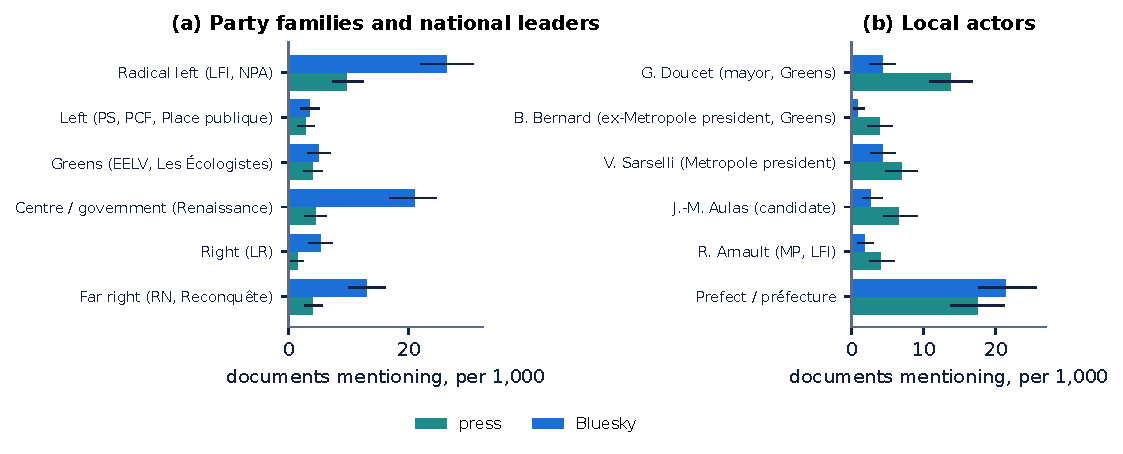
\includegraphics[width=\textwidth]{figures/f6_political_mentions.pdf}
\caption{Mentions of party families and national leaders (a) and of local actors (b), per 1,000 documents, with 95\% bootstrap intervals.}
\label{fig:politics}
\end{figure}

\paragraph{Framing of protests and riots.} We restrict the analysis to protest-related documents from 15 September (971 headlines, 895 posts). Figure~\ref{fig:frames} shows that Bluesky uses the \emph{far-right threat} lexicon (\emph{extr\^eme droite}, \emph{ultradroite}, \emph{n\'eonazis}, \emph{remigration}) 13 times more often than the press (172 versus 13 per 1,000) and the \emph{police repression} lexicon 16 times more often (98 versus 6). It also frames more in absolute terms. Among documents that carry at least one frame, the press relies mainly on \emph{order \& security} (43\% of framed headlines: \emph{casseurs}, \emph{d\'egradations}, \emph{forces de l'ordre}) and \emph{social grievance} (32\%), whereas half of the framed posts (51\%) invoke a far-right threat and 29\% police repression. The \emph{radical-left threat} frame is marginal in both sources. Within the press, Lyon Capitale gives more room to social grievance (48 per 1,000) and LyonMag to order and security (45 per 1,000). Several events show this difference: on 21 October, posts denounced a neo-Nazi march held in spite of the curfew (43 posts; no press headline uses the word), while headlines covered fines for curfew breaches and aid to shopkeepers.

\begin{figure}[htbp]
\centering
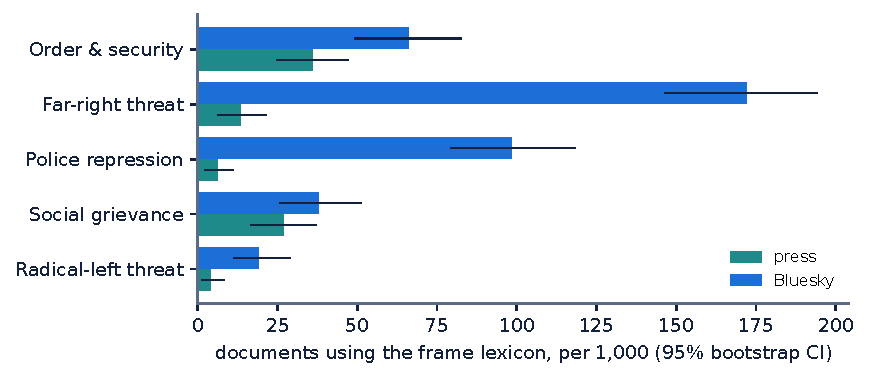
\includegraphics[width=0.75\textwidth]{figures/f7_frames.pdf}
\caption{Frame lexicons in protest-related documents (15 Sep -- 1 Nov), per 1,000 documents, with 95\% bootstrap intervals.}
\label{fig:frames}
\end{figure}

\paragraph{Distinctive vocabulary.} Table~\ref{tab:logodds} confirms these lexicon results with a data-driven method. In protest documents the press is distinctive through concrete damage and institutions (\emph{incendie}, \emph{pompiers}, \emph{commer\c{c}ants}, \emph{Doucet}), Bluesky through political qualification and national scope (\emph{extr\^eme droite}, \emph{r\'epression}, \emph{flics}, \emph{Paris}, \emph{Marseille}). In municipal politics the press names local leaders while Bluesky talks about irregularities and LFI. In the high-school movement the press counts blockaded schools and arrests while Bluesky expresses support and denounces repression.

\begin{table}[htbp]
\caption{Most distinctive words of each source within shared subsets (log-odds with informative Dirichlet prior~\cite{monroe2008fightin}; accents removed).}\label{tab:logodds}
\begin{tabularx}{\textwidth}{@{}lXX@{}}
\toprule
Subset & \press & \bsky \\
\midrule
Protests, riots, police & incendie, prison, lyceenne, doucet, etablissements, pompiers, emeutes, gregory, euros, presqu, commercants & paris, marseille, droite, manif, extreme, manifester, repression, images, nice, villes \\
Municipal politics & senatoriales, sarselli, doucet, aulas, bernard, gregory, bruno, veronique, judiciaire, denonce, sieges & politique, irregularites, marseille, maires, paris, annule, lfi, insoumis, insoumise \\
High-school movement & mobilisation, lyceenne, etablissements, interpellations, journee, blocage, lycees, direct, mortiers & soutien, repression, paris, manif, images, conditions, education, jeunesse \\
\botrule
\end{tabularx}
\end{table}

\paragraph{Sentiment.} Press headlines are more negative than posts: 55\% versus 40\% are classified negative, and mean polarity is $-0.23$ versus $-0.05$ ($\chi^2$ test, $p<10^{-50}$) (Figure~\ref{fig:sentiment}). This difference comes mostly from topic composition. Within shared topics the gap is small: on protests and on municipal politics the two sources are equally negative (mean negative probability 0.58 versus 0.61, and 0.54 versus 0.54; intervals include zero). Posts are slightly \emph{less} negative on police and court cases (0.76 versus 0.81) and on transport and regional news (0.48 versus 0.56). The only shared topic where posts are clearly more negative is weather and heat (0.42 versus 0.31), where users complain while forecasts stay factual. The press is not ``gloomier'' on the same subjects; it simply covers more accidents, fires and court cases.

\begin{figure}[htbp]
\centering
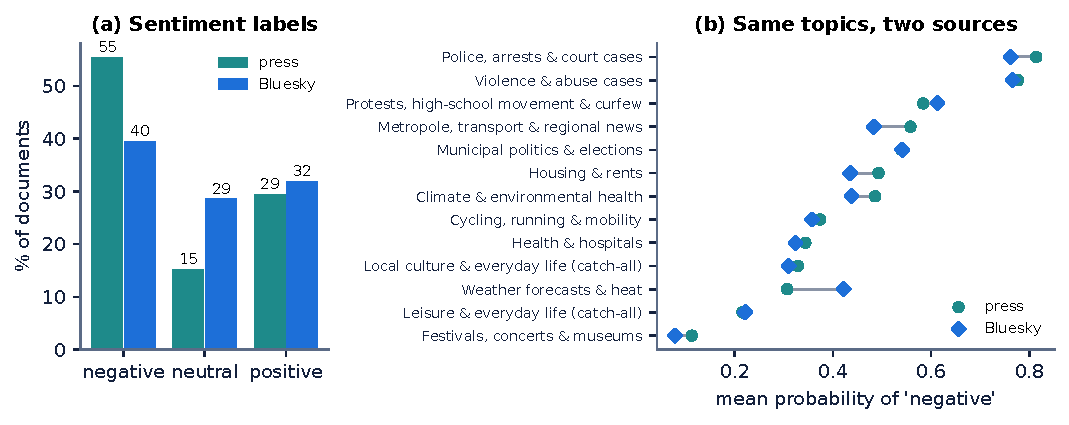
\includegraphics[width=\textwidth]{figures/f8_sentiment.pdf}
\caption{(a) Sentiment labels predicted by XLM-T. (b) Mean probability of negative sentiment for the same shared topics in each source.}
\label{fig:sentiment}
\end{figure}

\subsubsection{Discussion}

Our results nuance the idea that social networks ``scoop'' the press. At the scale of a city, both sources react to the same shocks within hours, and the press is often first for scheduled or institutional news. This is consistent with earlier findings on global newswire~\cite{petrovic2013newswire}, which found only small leads. What differs is \emph{selection} and \emph{framing}. The press covers many everyday incidents that never reach Bluesky. Bluesky turns local events into national political debates, with a lexicon centred on the far right and on police behaviour. This last point matches the left-leaning composition of Bluesky's audience reported by network studies~\cite{quelle2024bluesky}: our Bluesky corpus reflects a specific community, not ``the residents of Lyon''. We also showed how strongly corpus construction drives conclusions: one automated account would otherwise represent 40\% of the posts, and one ambiguous keyword (\emph{Rh\^one}) was enough to create a spurious Bluesky lead.

%% =====================================================================
\section{Conclusion}\label{sec:conclusion}

We built two comparable corpora on Lyon's local news, the press through raw GDELT files and Bluesky through its search API, and a reproducible pipeline that detects themes and emerging topics in each and compares them in a shared semantic space. Simple, explainable burst scores separate emerging from frequent topics (31 of the 32 top press terms match a real event). The two sources share most of their topical agenda and react to the same shocks within the same days, with no systematic lead. They differ in what they select (everyday incidents for the press, sport, culture and politics for Bluesky) and in how they frame the same events (local institutions and order for the press, national politics, the far right and police repression for Bluesky).

\subsection*{Contribution of each member}

\paragraph{Simon Hue.} Simon built the press part. He diagnosed the unusable GDELT API and replaced it by a collection from raw GKG ``translation'' files. He wrote the Lyon-area filter, the date correction and the coverage checks, and ran the exploratory analysis, the text analysis (PMI, log-odds), the K-Means and LDA comparison and the weekly outlet-weighted emergence score with its sensitivity analysis. He then carried out the cross-source analysis: re-collection of Bluesky with adaptive time splitting, refined territorial filter, joint BERTopic model, echo, synchrony, emergence lags, framing and sentiment. He also assembled this report. \emph{Most difficult:} obtaining usable data from GDELT and keeping the comparison fair despite a dominant regional paper, a coverage gap and automated accounts. \emph{Most interesting:} turning ``what is new?'' into a measurable quantity, and discovering that the two sources differ less in \emph{what} or \emph{when} than in \emph{how}.

\paragraph{L\'eo Marnas.} L\'eo built the streaming side of the Bluesky collection: a Jetstream collector that stores French-language posts in SQLite, applies edits and deletions, and reconnects after network failures. He wrote the preprocessing and exact de-duplication, and a suite of 20 unit tests covering collection, cleaning and analysis. He then integrated the Bluesky analysis into modular notebooks that reproduce the search-based pipeline exactly on a given corpus and report explicit diagnostics when a method cannot run (empty vocabulary, history too short, non-overlapping dates). \emph{Most difficult:} making a live collector reliable and reproducing an analysis exactly while the input data differed. \emph{Most interesting:} the AT Protocol data model and the constraints of a decentralised network.

\paragraph{Aaron Berton.} Aaron built the historical Bluesky collection with the search API (twelve Lyon keywords, day-by-day queries, resumable storage) and found and fixed the pagination bug. He designed the corpus rules (detection of automated accounts, per-account daily cap, de-duplication), the first BERTopic model on posts, the daily emergence detector with Jaccard-based event grouping, and the first design of the press--Bluesky comparison (semantic matching of topics, lagged correlations). \emph{Most difficult:} a feed dominated by one automated account and the pagination problem. \emph{Most interesting:} semantic topic modelling with sentence embeddings, which works where word-count models fail.

\subsection*{Limitations}

\begin{itemize}
\item \textbf{Coverage and representativeness.} Only three outlets are usable and one regional paper dominates; GDELT indexes part of their output and missed two days. Bluesky users are a specific, politically engaged and left-leaning community; the search API is not exhaustive and 12\% of the posts collected earlier were no longer available.
\item \textbf{Text.} We only have headlines for the press; full articles were not collected, out of respect for copyright and site terms.
\item \textbf{Time.} Thirteen weeks cover one season: seasonal and editorial declines cannot be separated, and events near the end of the window have unknown trajectories.
\item \textbf{Timing precision.} Press timestamps are GDELT detections (about one hour after publication) and day-level dates for some outlets.
\item \textbf{Models.} Topic partitions are only moderately stable across seeds (ARI 0.52--0.64 for the joint model, 0.25 for press K-Means), and topic labels are our interpretation. The emergence $z$ is a ranking index, not a calibrated p-value, as documents of one event are correlated and about 12,500 term-week tests are run.
\item \textbf{Framing.} Frame lexicons are hand-built and keyword-based (no negation, irony or stance), and mention counts do not reveal support or opposition. Manual annotations were done by a single annotator.
\end{itemize}

\subsection*{Perspectives}

Several extensions would strengthen these results: a second annotator and an inter-annotator agreement measure for events and echo pairs; a stance or frame classifier trained on a small labelled set instead of lexicons; a longer period (at least a year) to separate seasonal from editorial dynamics; more outlets (Rue89Lyon, Tribune de Lyon) collected from their own feeds; account-level analysis on Bluesky (communities of the follower graph) to tell which groups drive each frame; and full article text, where licences allow it, for finer topics.

\backmatter

\bmhead{Data and code availability} Code and aggregated outputs are in the project repository (\texttt{lyon-news-mining/}, \texttt{bluesky-news-mining/}, \texttt{cross-source/}). Raw Bluesky posts are kept locally and not redistributed; no personal handle is published in this report. The press corpus contains only GDELT metadata and headlines.

\bmhead{Use of AI assistance} Generative AI tools were used to help write code, draft parts of the text and produce a first annotation of the two evaluation samples (Section~\ref{sec:eval}); the annotation files are provided in the repository so that they can be checked. All analyses were run on our data.

\bibliography{references}

\end{document}
